\documentclass[11pt]{article}
\usepackage[letterpaper,margin=.25in]{geometry}
\usepackage{amsmath,amssymb,booktabs,array,tabularx,xcolor,tikz,hyperref,embedfile,microtype}
\usetikzlibrary{trees}
\hypersetup{colorlinks=true,urlcolor=blue!55!black}
\pagestyle{empty}
\setlength{\parindent}{0pt}
\setlength{\parskip}{4pt}
\linespread{1.035}\selectfont
\definecolor{navy}{RGB}{25,54,86}
\definecolor{soft}{RGB}{244,247,250}
\tikzset{branch/.style={circle,draw=navy,line width=.6pt,inner sep=2pt},trueleaf/.style={circle,draw=navy,fill=navy,inner sep=2.1pt},falseleaf/.style={circle,draw=navy,fill=white,inner sep=1.8pt}}
\newcommand{\sectionbar}[1]{\vspace{3pt}{\color{navy}\bfseries #1}\par\vspace{2pt}\hrule\vspace{4pt}}
\begin{document}
\enlargethispage{.12in}

\embedfile[desc={A120595 exact certificate payload},mimetype=application/json]{certificate_payload.json}
{\color{navy}\LARGE\bfseries A120595 concise calculus certificate}\hfill{\small VERIFIED}\\[-1pt]
{\small Bradley Klee, \quad Mech.An.ika Sol (Open AI) \hfill July 31, 2026}

\sectionbar{Definition and first terms}
\(\displaystyle 13\,A(x)=12+27\,x+A(x)^{4}\), with the origin-normalized solution.\\
{\footnotesize Normalization/grammar: \texttt{A(x)=1+(3)*T(x); T=x+2*T\textasciicircum{}2+4*T\textasciicircum{}3+3*T\textasciicircum{}4}.}\\
\(a(0),\ldots,a(7)=1,3,6,36,249,1932,16044,139500\).\\[2pt]
{\small Kernel used throughout: \(\displaystyle \rho(u)=u\,(1-2\,u^{1}-4\,u^{2}-3\,u^{3})\), so \(x=\rho(T(x))\).}

\sectionbar{Typogeometry}
\begin{minipage}[t]{.235\textwidth}\centering 
\begin{tikzpicture}[level distance=9mm,level 1/.style={sibling distance=10mm},level 2/.style={sibling distance=6mm},scale=.82,transform shape] \node[trueleaf] (n0) {};\end{tikzpicture}\\[2pt]{\normalsize\texttt{1x3}}\end{minipage}\begin{minipage}[t]{.235\textwidth}\centering 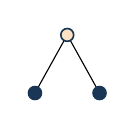
\begin{tikzpicture}[level distance=9mm,level 1/.style={sibling distance=10mm},level 2/.style={sibling distance=6mm},scale=.82,transform shape] \node[branch,fill=orange!24] (n0) {} child {node[trueleaf] (n1) {}} child {node[trueleaf] (n2) {}};\end{tikzpicture}\\[2pt]{\normalsize\texttt{\{1,1\}x6}}\end{minipage}\begin{minipage}[t]{.235\textwidth}\centering 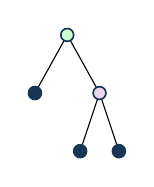
\begin{tikzpicture}[level distance=9mm,level 1/.style={sibling distance=10mm},level 2/.style={sibling distance=6mm},scale=.82,transform shape] \node[branch,fill=green!20] (n0) {} child {node[trueleaf] (n1) {}} child {node[branch,fill=violet!16] (n2) {} child {node[trueleaf] (n3) {}} child {node[trueleaf] (n4) {}}};\end{tikzpicture}\\[2pt]{\normalsize\texttt{\{1,\{1,1\}\}x12}}\end{minipage}\begin{minipage}[t]{.235\textwidth}\centering 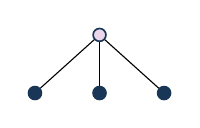
\begin{tikzpicture}[level distance=9mm,level 1/.style={sibling distance=10mm},level 2/.style={sibling distance=6mm},scale=.82,transform shape] \node[branch,fill=violet!16] (n0) {} child {node[trueleaf] (n1) {}} child {node[trueleaf] (n2) {}} child {node[trueleaf] (n3) {}};\end{tikzpicture}\\[2pt]{\normalsize\texttt{\{1,1,1\}x12}}\end{minipage}

{\footnotesize colored arity geometry; node color distinguishes constructors. Filled endpoints are true leaves; open endpoints are false/empty leaves. For colored grammars, color is genuine constructor data and is not silently converted into a positional zero pattern.}

{\footnotesize Typogeometric constructor codes and multiplicities: \(\Delta_{2}\!:\,2,\;\Delta_{3}\!:\,4,\;\Delta_{4}\!:\,3\).}

\sectionbar{Coefficient and contour extraction}
{\footnotesize \[\begin{gathered}\mathcal K_n=\{(k_1,\ldots,k_3)\in\mathbb Z_{\ge0}^{3}:\sum_{j=1}^{3}jk_j=n-1\},\quad K=\sum_{j=1}^{3}k_j,\\a(n)=\frac{3}{n}\sum_{\boldsymbol k\in\mathcal K_n}\binom{n+K-1}{K}\binom{K}{k_1,\ldots,k_3}2^{k_1} 4^{k_2} 3^{k_3}.\end{gathered}\]}
\(a(n)=\dfrac{3}{2\pi i n}\oint_\gamma\dfrac{du}{\rho(u)^n},\quad n\ge1.\)

\sectionbar{Recurrence}
{\footnotesize \(\sum_{r=0}^{3}P_r(n)a(n+r)=0\), \(n\ge 1\), with \[\begin{aligned}P_{0}(n)&=-6912\,n^{3} - 10368\,n^{2} - 1296\,n + 1080\\P_{1}(n)&=-9216\,n^{3} - 27648\,n^{2} - 26688\,n - 8256\\P_{2}(n)&=-4096\,n^{3} - 18432\,n^{2} - 26624\,n - 12288\\P_{3}(n)&=451\,n^{3} + 2706\,n^{2} + 4961\,n + 2706\end{aligned}\]}

\sectionbar{Differential equation}
{\footnotesize \[\left(1080\right)A(x)+\left(-18576\,x - 8256\right)A'(x)+\left(-31104\,x^{2} - 27648\,x - 6144\right)A^{(2)}(x)+\left(-6912\,x^{3} - 9216\,x^{2} - 4096\,x + 451\right)A^{(3)}(x)=0.\]}

\sectionbar{Matrices, telescoper certificate, and checks}
\begingroup\renewcommand{\arraystretch}{1.42}\setlength{\arraycolsep}{5pt}{\small\[\displaystyle U=\begin{pmatrix}\frac{3376}{451}&\frac{676}{451}&\frac{52}{451}&\frac{4}{451}\\\frac{8736}{451}&\frac{672}{451}&\frac{468}{451}&\frac{36}{451}\\\frac{8112}{451}&\frac{624}{451}&\frac{48}{451}&\frac{420}{451}\\0&0&0&0\end{pmatrix},\quad V=\begin{pmatrix}-1&0&0&0\\\frac{1572}{451}&\frac{225}{451}&\frac{52}{451}&\frac{4}{451}\\\frac{260}{41}&\frac{20}{41}&\frac{11}{41}&\frac{4}{41}\\\frac{2028}{451}&\frac{156}{451}&\frac{12}{451}&\frac{105}{451}\end{pmatrix},\quad J=\begin{pmatrix}0&1&0&0\\0&0&2&0\\0&0&0&3\\0&0&0&0\end{pmatrix}\]}\endgroup
\par\vspace{6pt}
{\small\textbf{Certificate.}\par\smallskip\(\displaystyle R(n,u)=N(n,u)/\rho(u)^{2},\ \deg_uN=9.\)\par}
\vspace{4pt}
{\small Telescoping identity: \(\sum_r P_r(n)H_{n+r}(u)=\partial_u\!\left(R(n,u)H_n(u)\right).\)\par}
\vspace{4pt}
{\footnotesize Matrix dimensions: \(8\times 8\); remainder \(3\times 4\), rank 3, nullity 1. The exact telescoping residual is zero. The recurrence reconstructs all 24 stored terms; 6/6 published OEIS prefix terms match.\par}

\vfill
\colorbox{soft}{\parbox{.97\textwidth}{\tiny Canonical records: \texttt{data/tree\_model.json}, \texttt{data/contour.json}, \texttt{data/matrices.json}, \texttt{data/recurrence.json}, \texttt{data/ode.json}. Embedded payload contains exact sources and SHA-256 matrix identifiers. Compare with the verbose certificate for A120590.}}
\end{document}
